\chapter{La reionisation } 
Nous avons vu dans le chapitre precedent que lors de la recombinaison, lunivers est passé d'un état globalement ionisé a un etat globalement neutre.
DE cette transition, qui a eu lieu a enciron 380000ans après le BB, en a resulté l'emission du CMB.
Suite a cette etape, l'univers etait alors homogene, et sa dinamique etait régie essentiellement par la lutte entre l'xpansion et la gravitation.
Du fait que l'univers etait neutre, le rayonnemenmt n'etait pas en mesure de se propager librement.
C'etait les ages sombres.

Il faudra alors attendre plusieurs centaine de million d'année pour voir apparaire des surdensité de gas suffisemment compactes pour former les première étoiles.
Ces premières sources lumineuses ont ont emmis un puissant rayonnement ionisant qui a a nouveau séparé les protons et les electron formé lors de la recombinaison.
Il a fallut encore plusieur centaine de million d'année pour que les première sources de rayonnement soient suffisement nombreuses pour que leurs photons remplissent l'univers, et le fasse passer d'un etat majoritairement neutre, a un etat a nouveau majoritairement ionisé. 
Cette transition s'appele l'epoque de la reionisation.



\section{Observation -> la reionization}

Une des difficultés de l'etude de la periode de reionization est que celle si a eu lieu tot dans l'histoire de l'univers lors de son premier milliard d'années.
Cette distance temporelle impose de regarder loin spatialement et donc de disposer de moyen observationnels important.
Nous somme au balbutiement des observation de la reionisation.
Dans cette section, je vais presenter quelqu unes des preuvent observationnelles de la reionisation. 


%le manque d'observations
%la difficulté des observations


\subsection{spectre de quasar}
Les quasars sont des objets tres brillants qui peuvent être observé a tres grandes distance.
Les plus lointains d'entre eux presentent  un tunnel gun peterson.

Lorsqu'un photon d'une energie proche 

\begin{figure}[bth]
        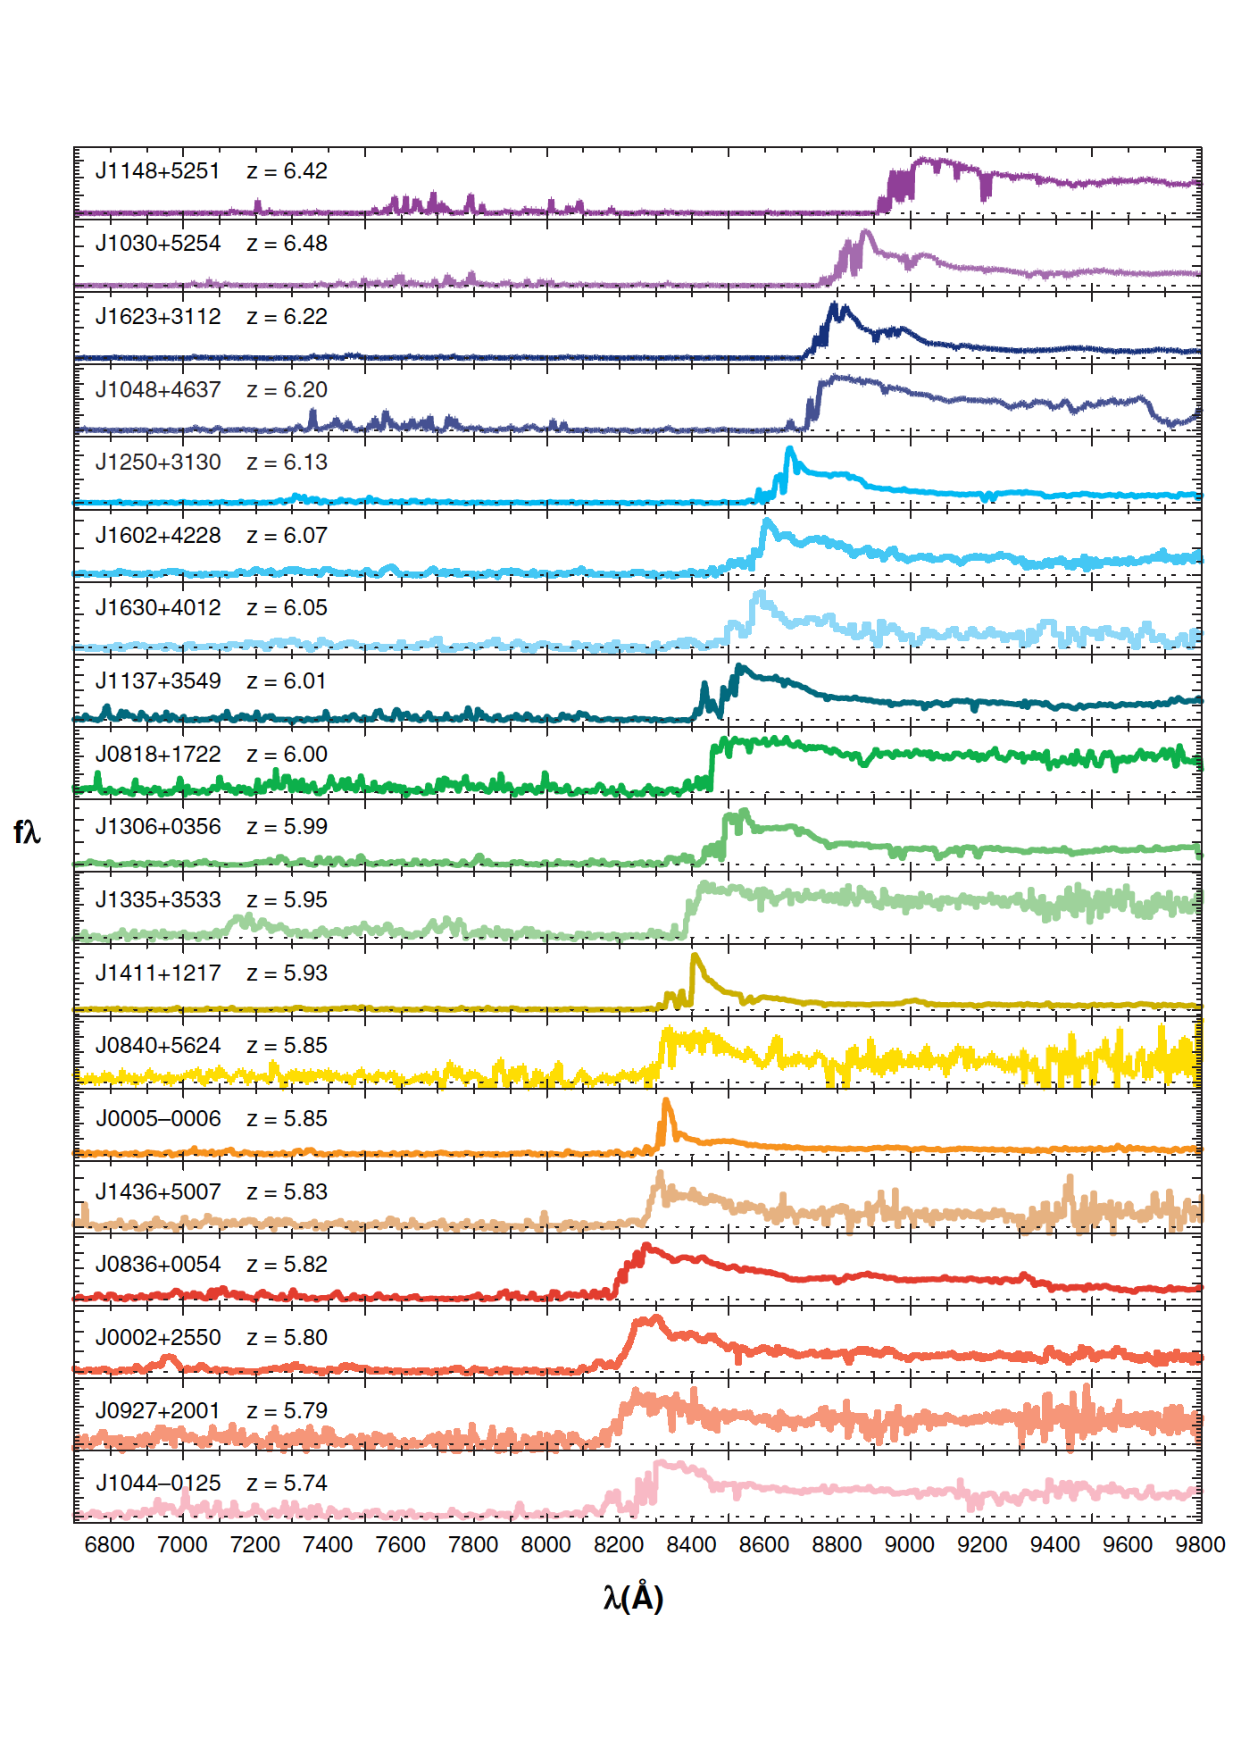
\includegraphics[width=.95\linewidth]{img/01/quasar_spectre.pdf} 
        \caption{Spectre de quasar a differents redshift presentant un tunnel gun peterson.
        Image fan et al.}
 		\label{fig:spectre_quasar}
\end{figure}

\subsection{Epaisseur optique lyman alpha}

\begin{figure}[bth]
        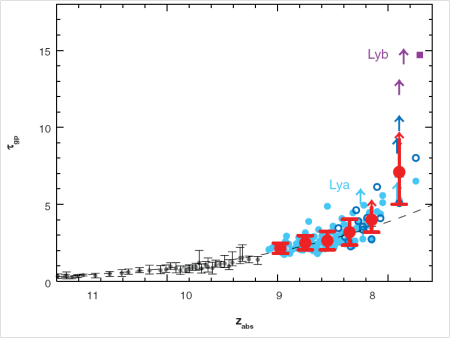
\includegraphics[width=.95\linewidth]{img/01/epaisseur_optique_quasar.png} 
        \caption{%https://ism2009.wordpress.com/2009/04/28/on-the-density-of-neutral-hydrogen-in-intergalactic-space/
		Epaisseur optique calculée a partir des spectres de quasar de la Fig\,\ref{fig:spectre_quasar}
        Image fan et al.}
 		\label{fig:epaisseur_optique_quasar}
\end{figure}

\subsection{Epaisseur optique lyman alpha}

\begin{figure}[bth]
        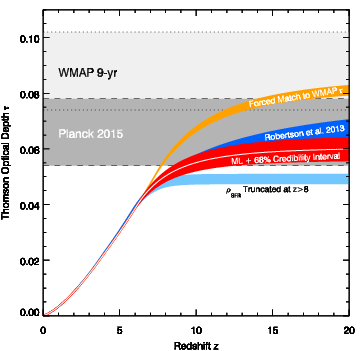
\includegraphics[width=.95\linewidth]{img/01/epaisseur_optique_thomson.png} 
        \caption{%https://inspirehep.net/record/1343310/plots
		Epaisseur optique Thomson
        Image Robertson et al.}
 		\label{fig:epaisseur_optique_thomson}
\end{figure}



\subsection{polarisation du CMB)}

\subsection{ligne 21 cm}

\subsection{fonction de luminosité UV}


\subsection{les futures observations}

Quelles sont les preuves de la réionisation?

\section{Théorie -> La reionization}

réionisation et non rayonnisation!

Qu'est ce que c'est?

fin des âges sombres
apparition des première sources de rayonnement
Pourquoi étudier la réionisation

Dernier processus impactant l'ensemble de l'univers.
Importance pour le "missing satellite problem"

\subsection{Sphère de Stromgren}


\subsection{les principales question en suspend de l'étude de la réionisation}

quand est ce arrivé?
quelles sont les sources? -> débat galaxies vs quasars
\begin{figure}[bth]
        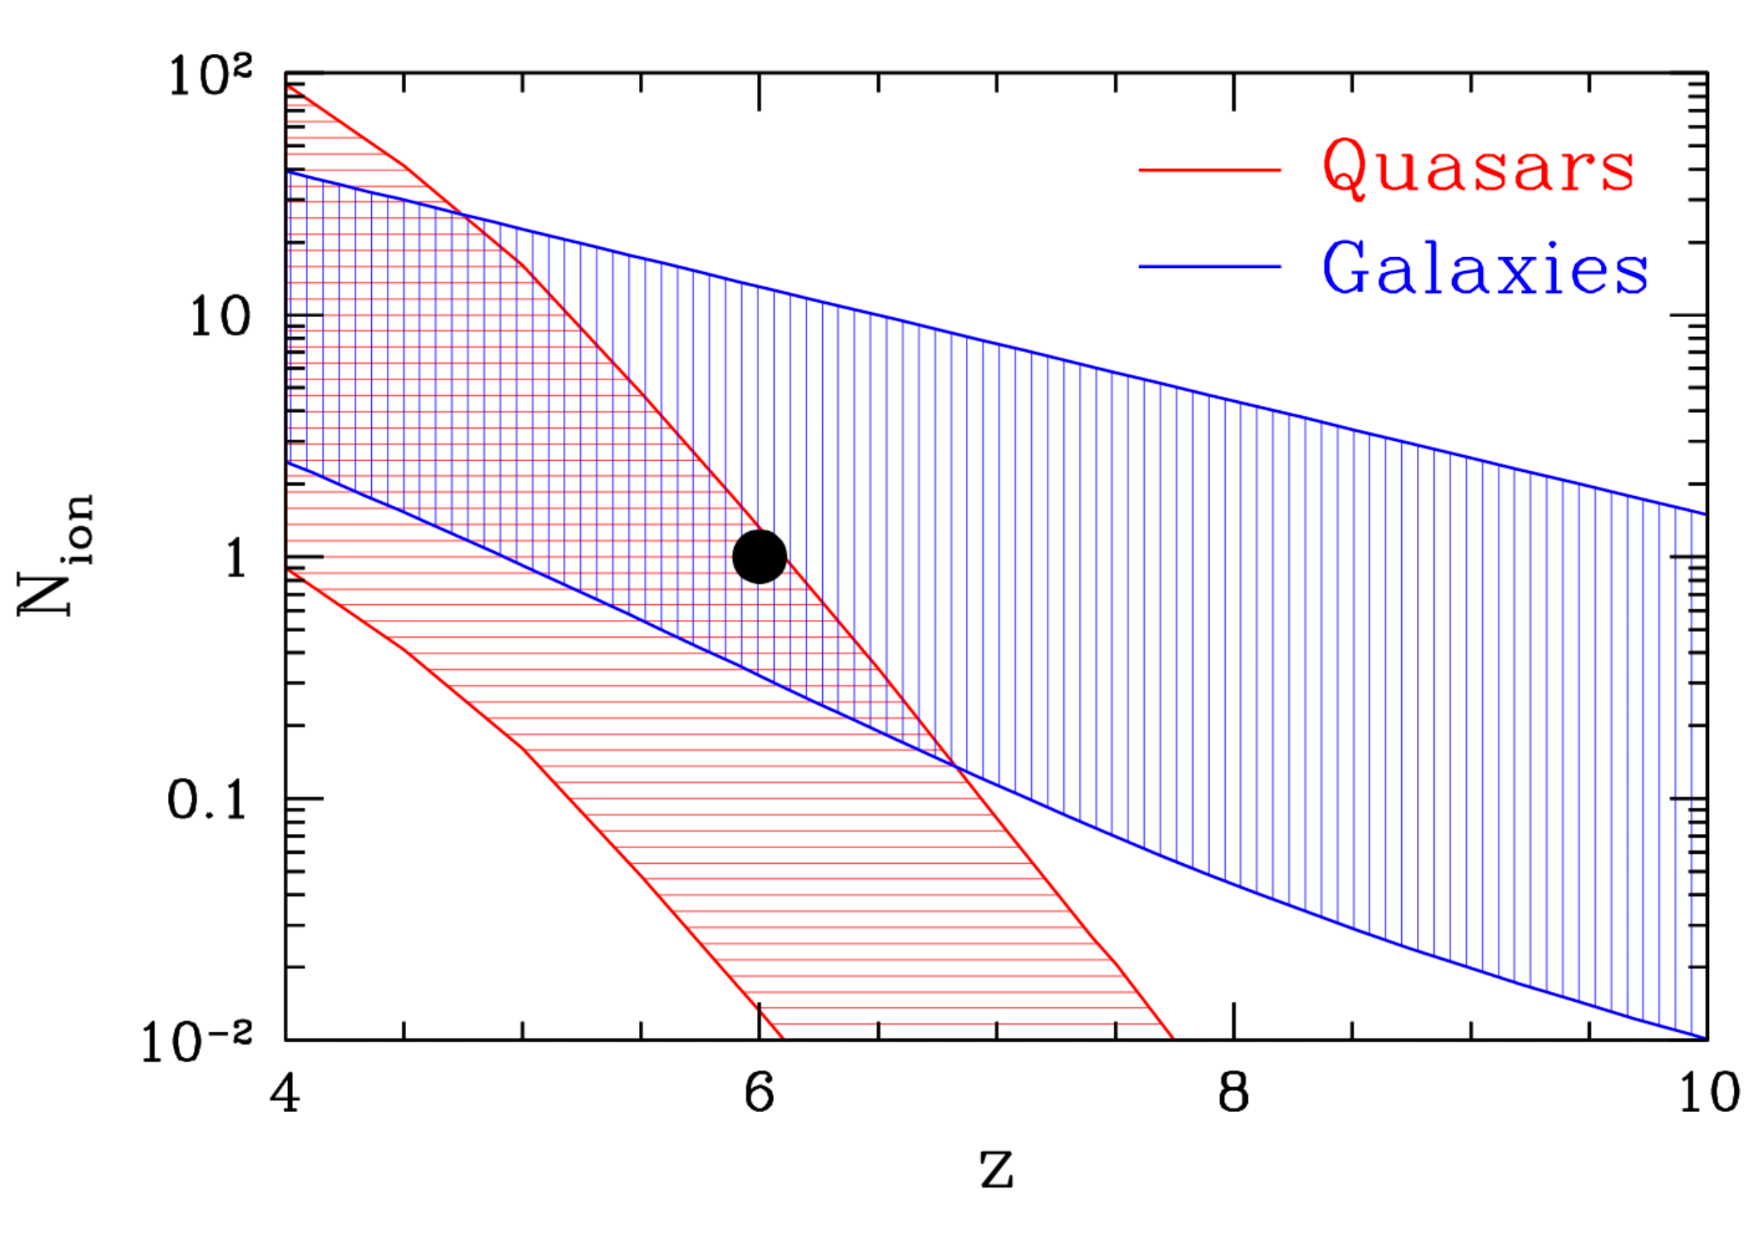
\includegraphics[width=.95\linewidth]{img/01/gal_AGN.pdf} 
        \caption{
        Budget de photons provenant des galaxies et des quasars qurant la reionization.
}
 		\label{fig:gal_AGN}
\end{figure}

outlier dans l'épaisseur optique des quasars
Le groupe local ?
